\let\negmedspace\undefined
\let\negthickspace\undefined
\documentclass[journal]{IEEEtran}
\usepackage[a5paper, margin=10mm, onecolumn]{geometry}

\usepackage{tfrupee}
\setlength{\headheight}{1cm}
\setlength{\headsep}{0mm}

\usepackage{gvv-book}
\usepackage{gvv}
\usepackage{cite}
\usepackage{amsmath,amssymb,amsfonts,amsthm}
\usepackage{algorithmic}
\usepackage{graphicx}
\usepackage{textcomp}
\usepackage{xcolor}
\usepackage{txfonts}
\usepackage{listings}
\usepackage{enumitem}
\usepackage{mathtools}
\usepackage{gensymb}
\usepackage{comment}
\usepackage[breaklinks=true]{hyperref}
\usepackage{tkz-euclide}
\usepackage{listings}

\def\inputGnumericTable{}
\usepackage[latin1]{inputenc}
\usepackage{color}
\usepackage{array}
\usepackage{longtable}
\usepackage{calc}
\usepackage{multirow}
\usepackage{hhline}
\usepackage{ifthen}
\usepackage{lscape}

\begin{document}
	
	\bibliographystyle{IEEEtran}
	\vspace{3cm}
	
	\title{2.5.16}
	\author{EE25BTECH11052 - Shriyansh Kalpesh Chawda}
	{\let\newpage\relax\maketitle}
	
	
	\renewcommand{\thefigure}{\arabic{figure}}
	\renewcommand{\thetable}{\arabic{table}}
	\renewcommand{\theequation}{\arabic{equation}}
	
	\textbf{Question:}\\
	Find the value of $p$ for which the lines are perpendicular.
	\[
	\frac{1-x}{3}=\frac{2y-14}{2p}=\frac{z-3}{2}
	\qquad\text{and}\qquad
	\frac{1-x}{3p}=\frac{y-5}{1}=\frac{6-z}{5}
	\]
	 \hfill (12, 2019)\\
\textbf{Solution:}\\
Writing each line in symmetric form to read off direction vectors.
		\begin{align}
	\vec{x} = \vec{A} + \lambda \vec{m}
		\end{align}
		From
	\begin{align}
	\frac{1-x}{3}=t,\;
	\frac{2y-14}{2p}=t,\;
	\frac{z-3}{2}=t,
	\end{align}
	we obtain
\begin{align}
	x = 1-3t,\quad
y = 7+pt,\quad
z = 3+2t.
\end{align}
Hence, the direction vector is
	\begin{align}
		\vec{m_1} = \myvec{-3\\ p\\ 2}
	\end{align}
From
\begin{align}
	\frac{1-x}{3p}=s,\;
\frac{y-5}{1}=s,\;
\frac{6-z}{5}=s,
\end{align}
we obtain
	\begin{align}
			x = 1-3ps,\quad
		y = 5+s,\quad
		z = 6-5s.
	\end{align}
	Hence, the direction vector is
	\begin{align}
		\vec{m_2} = \myvec{-3p\\ 1\\ -5}
	\end{align}
The lines are perpendicular when
	\begin{align}
		\vec{m_1}^\top \vec{m_2} &= 0
	\end{align}
	Substituting from (4) and (7),
	\begin{align}
		\myvec{-3 & p & 2}\myvec{-3p\\[2pt] 1\\[2pt] -5} &= 0 \\
		(-3)(-3p) + p\cdot 1 + 2(-5) &= 0 \\
		9p + p - 10 &= 0 \\
		10p - 10 &= 0 \\
		\Longrightarrow\; p &= 1
	\end{align}
Therefore, the required value is
$$
	\boxed{p=1}
$$
The plot of the two lines are show in the plot below :
\begin{figure}[H]
	\centering
	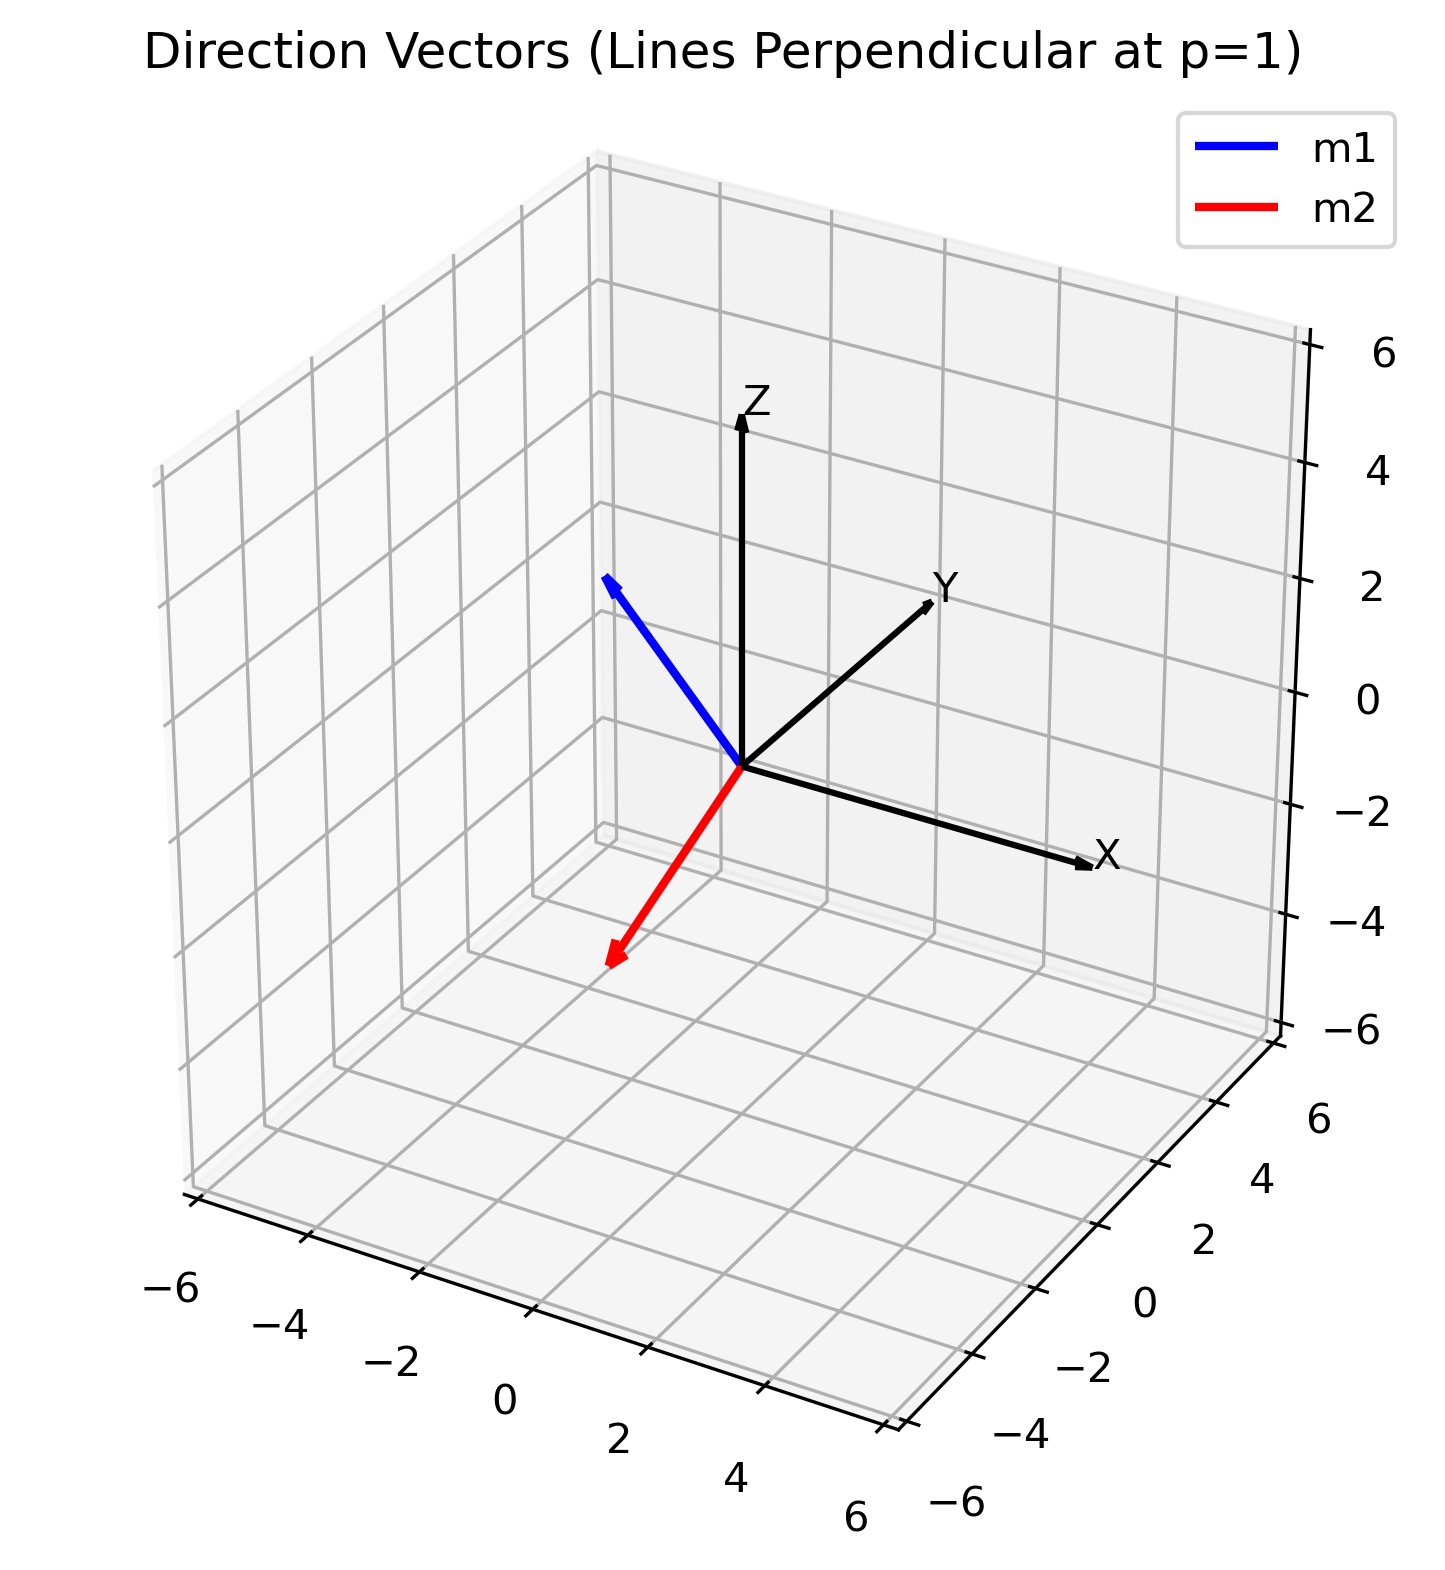
\includegraphics[width=0.8\linewidth]{figs/equations_solution}
	\caption{}
	\label{fig:equationssolution}
\end{figure}

	
\end{document}
